\documentclass[11pt, spanish]{article}

\usepackage[spanish]{babel}
\selectlanguage{spanish}
\usepackage[utf8]{inputenc}
\usepackage{graphicx}
\usepackage{amsmath, amssymb}
\usepackage{enumerate}
\begin{document}

\section{Cálculo de probabilidades de eventos (Diagrama de Venn)}

Petrocol es una multinacional dedicada a la producción de petróleo que opera en Colombia. El plan estratégico de la compañia contempla la inversión en exploración y explotación de nuevos yacimientos. En este plan existen dos alternativas de inversión que son atractivas económicamente para la junta directiva. La primera alternativa (\textbf{Alternativa A}) consiste en explorar y explotar las reservas de petróleo ubicadas en aguas profundas del caribe colombiano. La segunda alternativa (\textbf{Alternativa B}) consiste en explorar y explotar las reservas petroleras distribuidas en los municipios de Arauca y Casanare. Petrocol reconoce que, por restricciones presupuestarias, no cuenta con los recursos operativos (maquinaria y equipo) suficientes para implementar las dos alternativas de manera simultánea. Esto implica que se debe elegir cuál de las dos alternativas se implementará primero. Adicionalmente, la junta directiva está considerando varias alternativas de financiación para respaldar el proyecto que se elija. Estas alternativas de financiación son:

\begin{itemize}
\item \textbf{Crédito Bancario}: obtener el 100\% de los recursos económicos que requiere la alternativa a través de un crédito.
\item \textbf{Exceso de Caja}: financiar la totalidad del proyecto de contado, a partir del exceso de caja que se obtuvo el año anterior.
\item \textbf{Emisión de Acciones}: realizar una emisión de acciones para recaudar el capital necesario de la alternativa.
\end{itemize}

Con el fin de analizar las dos alternativas de inversión, la junta directiva realizó una encuesta a 5000 accionistas de la compañía, seleccionados de manera aleatoria. La junta directiva espera que la encuesta les permita evaluar las preferencias de los accionistas en cuanto al proyecto que se debería realizar y al método de financiación que considerarían apropiado. Los resultados de la encuesta arrojaron la siguiente información:

\begin{itemize}
\item 2320 accionistas están de acuerdo con la inversión en la alternativa A.
\item 745 accionistas no están de acuerdo con el plan estratégico de la junta directiva.
\item 1690 accionistas están de acuerdo en invertir en la alternativa A y financiarla a partir de un crédito bancario. De esos 1690, hay 865 que también aceptarían utilizar el exceso de caja
como forma de financiación.
\item 185 accionistas están de acuerdo con invertir en la alternativa B y consideran que la opción 3 es el único método de financiación adecuado.
\item De los accionistas que apoyan la alternativa B y que consideran apropiado utilizar el exceso
de caja, hay 145 que también estarían dispuestos a aceptar una emisión de acciones, pero
que no aceptarían solicitar un crédito bancario.
\item 1285 accionistas están de acuerdo con invertir en la alternativa B y financiarla a partir de un
crédito bancario. De estos 1285, 610 también estarían de acuerdo con una emisión de acciones; y de los 610, son 200 los accionistas que también estarían de acuerdo con utilizar el exceso de caja.
\item De los 1285 accionistas que financiarían la alternativa B con un crédito bancario, hay 315 que estarían también de acuerdo con utilizar el exceso de caja pero no estarían de acuerdo con una emisión de acciones.
\item De los accionistas que apoyan la alternativa A, ninguno de ellos considera que una emisión de acciones es un método viable de financiación.

\end{itemize}

Con base en la información anterior, de respuesta a los siguientes literales:

\begin{enumerate}[(a)]

\item Con base en la información anterior, mencione los eventos que se presentan en la situación expuesta.\\

Los eventos presentados en la descripción del problema anterior, incluyen los eventos asociados al lugar de a inversión y los tipos de inversión. Es decir, los eventos probables de éste experimento es el producto cruz de las alternativas y los métodos de inversión ($CB$ representa crédito bancario, $EC$, emisión de caja y $EA$ emisión de acciones). Sin embago, es necesarios tener en cuneta que los accionistas que apoyan la alternativa A no desean financiar el proyecto através de emisión de caja:

$$\Omega = \left[A, B \right] \times \left[CB, EC, EA \right]$$
$$\Omega = \left\{ (A, CB), (A, EA), (B, CB), (B, EC), (B, EA)\right\}$$

\pagebreak

\item Realice un diagrama de Venn que indique la cantidad de accionistas que pertenecen a cada evento.\\

\begin{figure}[h]
\centering
	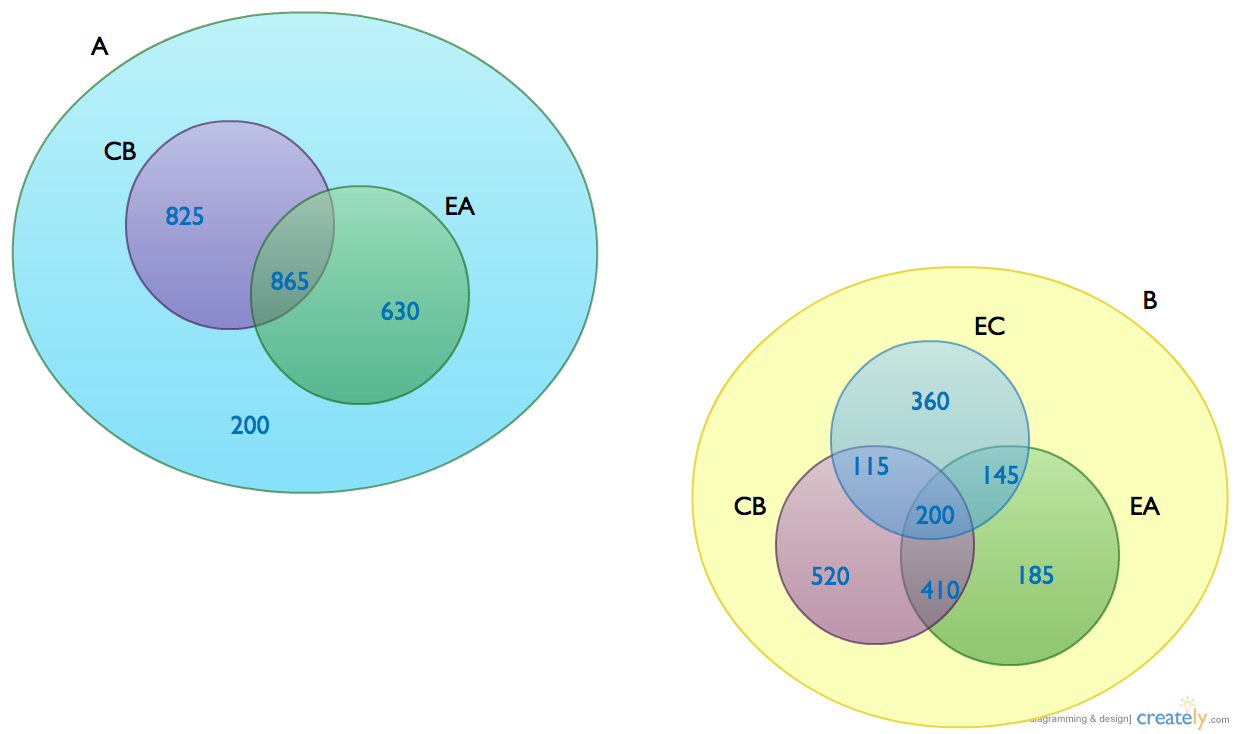
\includegraphics[scale=0.3]{venn_diagram.png}
	\caption{Diagrama de Venn para la representación de probabilidades}
\end{figure}

Las principales cardinalidades para el cálculo de probabilidades son:

$$\left| \Omega \right| = 5000\ \left| A \right| = 2320\ \left| B \right| = 1935\ \left| B^{c} \cap A^{c} \ \right| = 745$$

\item Cuál es la relación entre los eventos, financiarse vía emisión de acciones e invertir en la alternativa B.\\

Los eventos no son mutuamente excluyentes, la probabilidad de su intrsección no es vacía.

$$P(B) = \frac{\left| B \right|}{\left| \Omega \right|} = \frac{1935}{5000} = 0.387$$

$$P(EA) = \frac{\left|  EA \right|}{\left| \Omega \right|} = \frac{\left|  EA \cap A \right| + \left|  EA \cap B \right|}{5000} = \frac{2435}{5000} = 0.487$$

$$P(EA \cap B) = \frac{\left|  EA \cap B \right|}{\left| \Omega \right|} = \frac{185 + 410 + 200 + 145}{5000} = \frac{940}{5000} = 0.188$$

Los eventos son independientes, pues:

$$P(B)P(EA) = 0.387 \times 0.487 = 0.188 = P(B \cap EA)$$

\item Si se tienen los eventos A y B relacionados con que un accionista esté de acuerdo en invertir en la alternativa A o B, ¿se podría afirmar que estos eventos son independientes? Justifique su respuesta.\\

Los eventos no son independientes, para esto, se listan las probabilidades necesarias:

$$P(A) = \frac{\left| A \right|}{\left| \Omega \right|} = \frac{2320}{5000} = 0.464$$

$$P(B) = \frac{\left| B \right|}{\left| \Omega \right|} = \frac{1935}{5000} = 0.387$$

$$P(B \cap A) = \frac{\left| B \cap A \right|}{\left| \Omega \right|} = \frac{0}{5000} = 0$$

$$P(B \cap A) \neq P(A)P(B)$$

Luego, los eventos no son independientes

\item Calcule la probabilidad de que el accionista esté de acuerdo con invertir en la alternativa B.\\

$$P(B) = \frac{\left| B \right|}{\left| \Omega \right|} = \frac{1935}{5000} = 0.387$$

\item Calcule la probabilidad de que el accionista esté de acuerdo con invertir en la alternativa A y en la alternativa B.\\

$$P(B \cap A) = \frac{\left| B \cap A \right|}{\left| \Omega \right|} = \frac{0}{5000} = 0$$

\item Calcule la probabilidad de que el accionista esté de acuerdo con financiarse vía préstamo bancario.\\

$$P(CB) = \frac{\left| CB \right|}{\left| \Omega \right|} =  \frac{\left| CB \cap A \right|}{\left| \Omega \right|} + \frac{\left| CB \cap B \right|}{\left| \Omega \right|} = 0.587$$

\item Calcule la probabilidad de que el accionista esté de acuerdo con invertir en la alternativa A y que tenga preferencias por obtener un crédito bancario y usar el exceso de caja como posibles métodos de financiación.\\

$$P(A \cap CB \cap EC) = \frac{\left| A \cap CB \cap EC \right|}{\left| \Omega \right|} = \frac{865}{5000} = 0.173$$

\item Calcule la probabilidad de que el accionista esté de acuerdo con financiarse únicamente con una emisión de acciones.\\

Sean los eventos $EA_{A}$ y $EA_{B}$ los eventos que toman sólo la porción que desea invertir únicamente en $EA$ en $A$ y en $B$ respectivamente. $EA_{A} = A \cap (EA \char`\\ (EA \cap CB))$ y $EA_{B} = B \cap (EA \char`\\ (EA \cap CB) \char`\\ (EA \cap EC)$. Se pide la probabilidad de elegir únicamente e tipo $EA$ de financiación, se nombra este evento como $EA_{*}$.

$$P(EA_{*}) = \frac{\left| EA_{*} \right|}{\left| \Omega \right|} = P(EA_{A}) + P(EA_{B}) = \frac{630}{5000} + \frac{185}{5000} =  0.163$$

\item Calcule la probabilidad de que el accionista esté de acuerdo invertir en la alternativa B y tenga preferencias únicamente por dos de los tres métodos de financiación.
$$P(B \cap (CB \cup EC)) + P(B \cap (EA \cup EC)) + P(B \cap (CB \cup EA)) = 0.134$$

\item Si se sabe que el accionista prefiere la inversión en la alternativa B, ¿cuál es la probabilidad de que el accionista tenga preferencias únicamente por las opciones de financiación vía emisión de acciones y préstamo bancario?\\

$$P(EA \cap CB | B) = \frac{\left| EA \cap B \right|}{\left| B \right|} =  \frac{410}{1935} =  0.211$$

\item Si se sabe que el accionista prefiere financiar el proyecto vía préstamo bancario, ¿cuál es la probabilidad de que el accionista esté de acuerdo en invertir en la alternativa A?\\

$$P(A | CB) = \frac{P(A \cap CB)}{P(CB)} =  \frac{0.338}{0.587} =  0.575$$
\end{enumerate}

\section{Cálculo de probabilidades de eventos (Gráficas)}

Se dispone de un sistema eléctrico que está conformado por 6 componentes, tal como se ilustra en la Figura 2. Este sistema funciona si es posible enviar corriente desde la entrada del sistema hasta su salida. La probabilidad de que cada uno de los componentes funcione apropiadamente es independiente de los demás componentes, y su valor se presenta en la figura que se muestra a continuación, entre paréntesis.

\begin{figure}[h]
\centering
	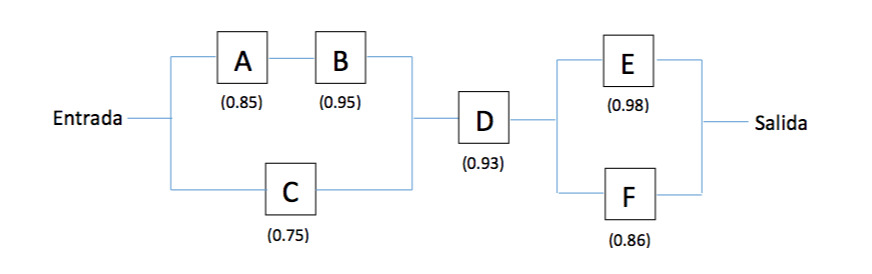
\includegraphics[scale=0.8]{circuit.png}
	\caption{Sistema eléctrico}
\end{figure}

Tenga en cuenta que un sistema en serie funciona si todos sus componentes funcionan; y que un sistema en paralelo funciona si por lo menos uno de los componentes, o serie de componentes, funciona. Con base en la información anterior, responda la pregunta enunciada en el literal $a$.

\begin{enumerate}[(a)]
\item Calcule la probabilidad de que el sistema eléctrico funcione. Sea explícito con el uso de fórmulas, eventos, uniones e intersecciones.\\

Para el desarrollo de este ejercicio, se propone como estrategia reducir cada subsistema mostrado en la Figura 3, y luego hallar la probabilidad de funcionamiento del sistema. Los subsistemas se muestran a continuación.

\begin{figure}[h]
\centering
	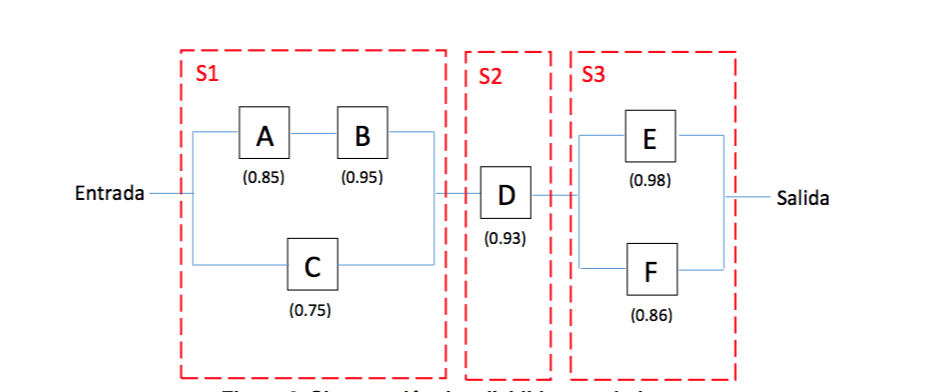
\includegraphics[scale=0.8]{subsystems.png}
	\caption{Sistema eléctrico}
\end{figure}

Para hallar la probabildad de funcionamiento de $S_{1}$, se debe hallar la probabilidad del funcionamiento en serie de $A$ y $B$. A continuación, se halla la probabilidad de funcionamiento de este nuevo bloque con el bloque $C$ en paralelo. El nuevo bloque llamado $A \cap B$, tiene como probabilidad de funcionamiento $P(A \cap B)$. Como cada bloque es independiente, $P(A \cap B) = P(A)P(B)$. Ahora como un sistema en paralelo depende del funcionamiento de al menos uno de los bloques que lo componen, se halla la probabilidad de funcionamiento de los bloques $C$ y $A \cap B$ en paralelo. La probabilidad de funcionamiento de el nuevo bloque llamado $C \cup (A \cap B)$ es $P(C \cup (A \cap B))$, esta probabilidad, se halla con los complementos, es decir, $P(C \cup (A \cap B)) = 1 - P(C^c \cap (A \cap B)^c)$, ya que los eventos son independientes, se tiene $P(C^c \cap (A \cap B)^c) = P(C^c)P((A \cap B)^c)$, esto por la ley de complementos, equivale a $(1 - P(C))(1 - P(A \cap B))$. $P(C \cup (A \cap B)) = P(S_{1})$.

$$P(A \cap B) = P(A)P(B) = (0.85)(0.95) = 0.8075$$
$$P(AB \cup C) = 1 - P(AB^c \cap C^c) = 1 - P(AB^c)P(C^c)$$
$$P(AB \cup C) = 1 - (1 - P(AB))(1 - P(C)) = 1 - (1-0.8075)(1-0.75) = 0.952$$
$$P(S_{1}) =  0.952$$

La probabildad de que el sistema 2 funcione, $P(S_{2})$, es $P(S_{2}) = P(D) = 0.93$. Para el tercer sistema $S_{3}$, se cuenta con dos bloques en paralelo, es decir:

$$P(S_{3}) = P(E \cup F) = 1 - P(E^c \cap F^c) = 1 - P(E^c)P(F^c)$$
$$1 - P(E^c)P(F^c) = 1 - (1 - P(E))(1 - P(F))$$
$$P(S_{3}) =  1 - (1 - 0.98)(1 - 0.86) = 0.997$$

Con las tres probabilidades, $P(S_1), P(S_2), P(S_3)$, se calcula la probabilidad de funcionamiento del sistema. 

$$P(S) = P(S_1 \cap S_2 \cap S_3) = P(S_1)P(S_2)P(S_3) = 0.952 \times 0.93 \times 0.997 =  0.883$$

\end{enumerate}

\section{Técnicas de Conteo}

El próximo torneo de fútbol al que fue invitada la Universidad de los Andes se llevará a cabo en el mes de octubre, y en él competirán 8 equipos. Para este torneo, la Universidad de los Andes contará con la presencia de sus mejores cuatro equipos, pertenecientes a las facultades de Ingeniería, Administración, Derecho y Matemáticas. Los restantes cuatro equipos, provenientes de otras universidades, pertenecen a las facultades de Ingeniería, Comunicación, Psicología y Diseño.\\

Los organizadores del torneo aún no han informado cuál es el sistema de eliminación, sin embargo, usted supone que se implementará un sistema de puntos en el que todos juegan contra todos. Conteste las siguientes preguntas bajo el supuesto de que es un torneo en el que todos juegan
contra todos.

\begin{enumerate}[(a)]
\item ¿Cuántos resultados posibles se pueden dar en términos de los puestos obtenidos
por cada equipo?

\item ¿Cuál es la probabilidad de que el primer y el segundo puesto sean ocupados por
equipos de los Andes?

\item ¿Cuál es la probabilidad de que los tres primeros lugares sean ocupados por equipos
de las facultades de Comunicación, Derecho y Administración (sin importar el orden)?

\item ¿Cuál es la probabilidad de que el primer lugar sea ocupado por un equipo de
Ingeniería, el segundo por el de Matemáticas y el tercero por el de Diseño?
\end{enumerate}

Su otro supuesto sobre el sistema de eliminación consiste en que se organizarán dos grupos de
cuatro equipos, y se realizará una ronda final entre los ganadores de cada uno de los grupos. Bajo
este supuesto, de respuesta a las siguientes preguntas.

\begin{itemize}
\item[(e)] ¿De cuántas formas distintas se podrían organizar los 8 equipos en dos grupos?

\item[(f)]  ¿Cuál es la probabilidad de que en un mismo grupo quede únicamente un equipo de
Ingeniería y el equipo de Diseño?

\item[(g)]  Si se supone que los cuatro equipos representantes de la Universidad de los Andes
quedan en el mismo grupo ¿Cuál es la probabilidad de que los equipos de las facultades de
Ingeniería queden de primeros en cada grupo?
\end{itemize}


\end{document}